\chapter{Verbetering van een keyword tool}
\label{ch:tool}

\section{Motivatie}
\label{ch: Motivatie}

Een zoekwoordonderzoek bestaat er onder andere in alle gevonden zoekwoorden onder te verdelen in groepen of clusters. Om het concept  'clusters' te verduidelijken, werken we met een voorbeeld.

Wanneer we bepaalde gerelateerde zoekwoorden en hun zoekvolume te zien krijgen, ziet dit er als volgt uit (wanneer we zoeken op ‘restaurant Brugge’): 

\begin{figure}[h!]
\centering
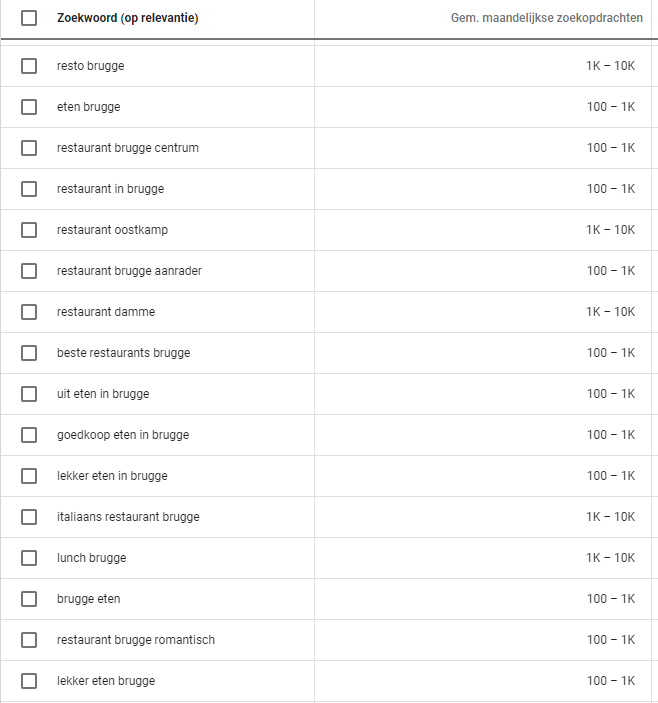
\includegraphics[width=0.8\textwidth]{img/Keywordplannervoorbeeld.png}
\caption{Screenshot van de Zoekwoordplanner die zoekwoordsuggesties geeft voor het zoekwoord 'restaurant Brugge'}
\end{figure}

Er zijn vaak honderden, soms zelfs duizenden zoekwoorden. Om meer overzicht te krijgen hierin, is het een goed idee om dezelfde patronen te groeperen. De zoekwoorden ‘eten Brugge’, ‘uit eten in Brugge’ en ‘Brugge eten’ behoren allemaal tot dezelfde groepering (omdat de intenties van het zoekwoord dezelfde zijn). Van deze zoekwoorden kan je dan een clustergroep maken (van alle mensen die willen eten in Brugge). Die ziet eruit als volgt:

Clustergroep: eten Brugge
eten Brugge - 880
Brugge eten - 390
uit eten in Brugge - 1000

Er bestaan uiteraard nog meer  clustergroepen voor relevante woorden van het keyword ‘restaurant Brugge’. 

Met de zoekwoorden uit deze clustergroepen kan je uiteindelijk landingspagina’s (een pagina op een website) gaan maken, die deze woorden bevatten. Over het algemeen wordt er per clustergroep een landingspagina opgesteld.  

Bij WiSEO gebeurt dit telkens handmatig door middel van Spreadsheets, waarbij alles manueel overgetypt wordt. Vanuit de zoekwoordtool (zie bovenstaande foto) wordt alles één voor één overgenomen. Een voorbeeld van het resultaat: 

\begin{figure}[h!]
\centering
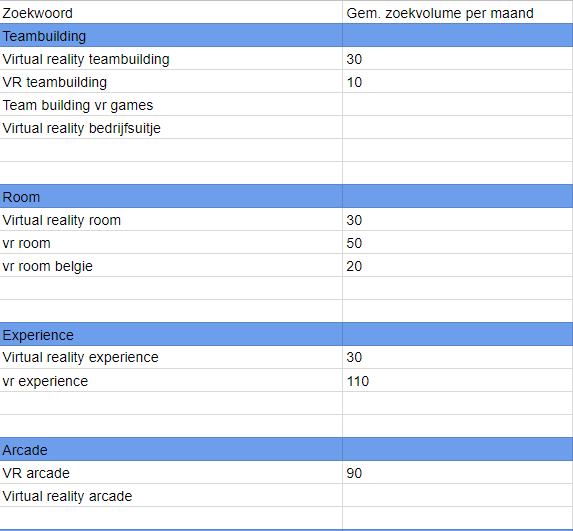
\includegraphics[width=0.8\textwidth]{img/Clustergroepenvoorbeeld.png}
\caption{Voorbeeld van clustergroepen in een Excel bestand}
\end{figure}

\newpage
\section{Aanpak}
\label{ch: Aanpak}

WiSEO's idee was om een eigen tool te programmeren zodat het proces vergemakkelijkt wordt (en dus minder tijd in beslag neemt), met als doel het handmatige proces van kopiëren en plakken achterwege te laten. 

De werking van deze tool werd gebaseerd op een reeds bestaande tool, namelijk Kwfinder. Het is de bedoeling om een zoekwoord samen in te geven met een bepaald land en een bepaalde taal, om op die manier suggesties te krijgen van gerelateerde zoekwoorden en hun maandelijks zoekvolume. Bij Kwfinder ziet dit er als volgt uit: 

\begin{figure}[h!]
\centering
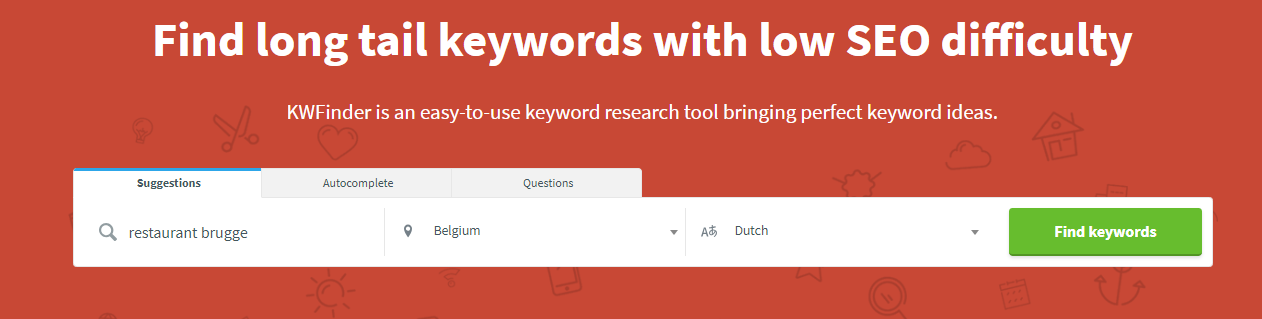
\includegraphics[width=0.8\textwidth]{img/kwfindervoorbeeld.png}
\caption{Screenshot 1 van de tool Kwfinder}
\end{figure}

Na op de knop ‘Find keywords’ te klikken, verkrijg je het volgende resultaat: 

\begin{figure}[h!]
\centering
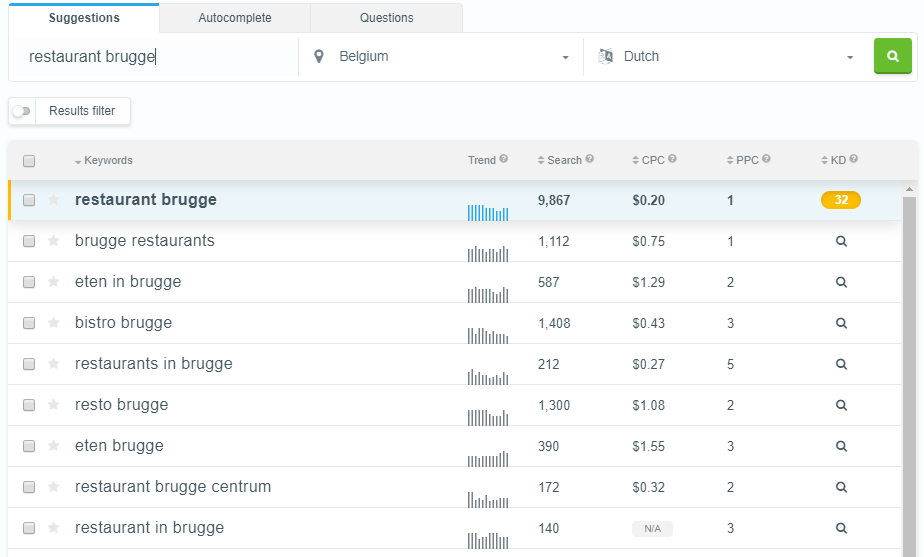
\includegraphics[width=0.8\textwidth]{img/kwfindervoorbeeld2.png}
\caption{Screenshot 2 van de tool Kwfinder}
\end{figure}

De zoekwoordsuggesties en zoekvolumes zijn nu zichtbaar, deze moeten geclusterd worden. De linkerkant van het programma wordt gebaseerd op de bovenstaande foto. 

Clusters en hun zoekwoorden worden ingegeven aan de rechterkant van het programma. Door de zoekwoorden te selecteren (links) kan je ze aan de rechterkant samenvoegen met het zoekvolume in een aangemaakte cluster. 

Om alles te verduidelijken is hieronder een mock-up te vinden van hoe het programma er uit zal zien. Deze mock-ups zijn vooraf gemaakt om het verschil te laten zien tussen het initieel ontwerp en het uiteindelijke product. 

\newpage
Hier kan je een zoekwoord ingeven met een land en taal naar keuze om zo gerelateerde keywords en het zoekvolume te verkrijgen: 

\begin{figure}[h!]
\centering
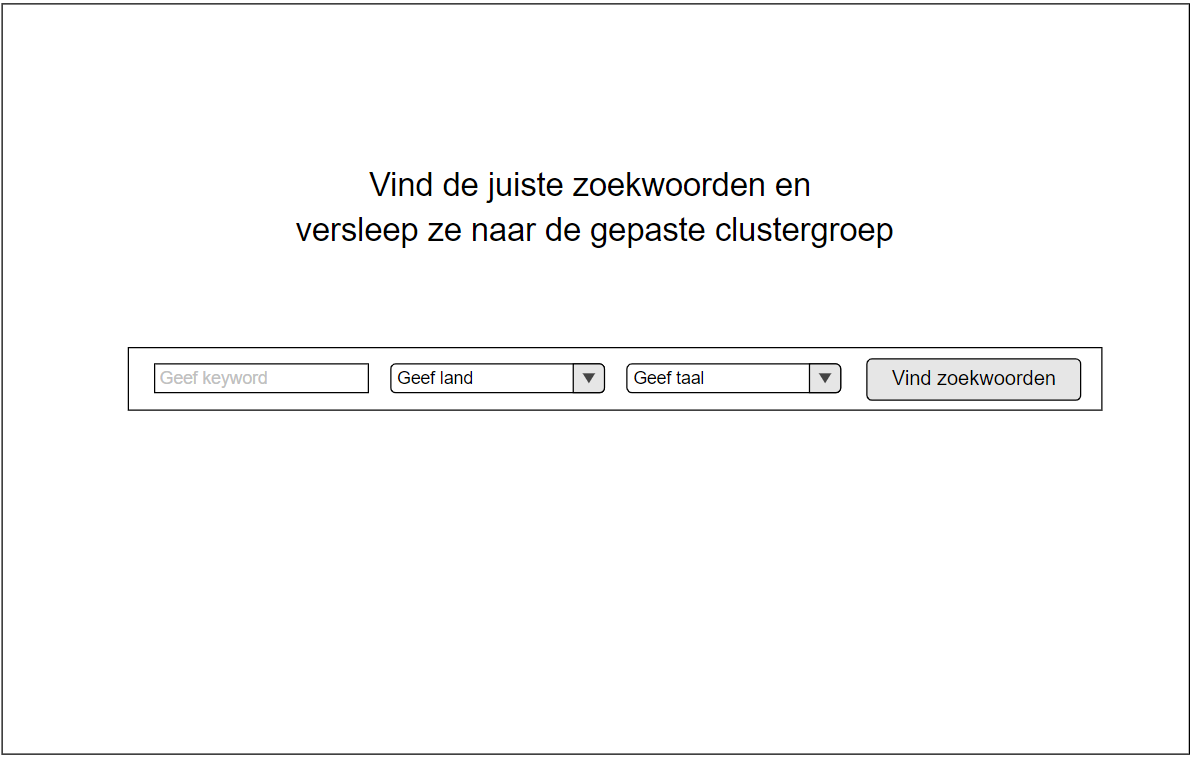
\includegraphics[width=0.8\textwidth]{img/Mockup.png}
\caption{Screenshot van mock-up 1}
\end{figure}

Na op de knop ‘Vind zoekwoorden’ te klikken, verkrijg je het volgende resultaat: 

\begin{figure}[h!]
\centering
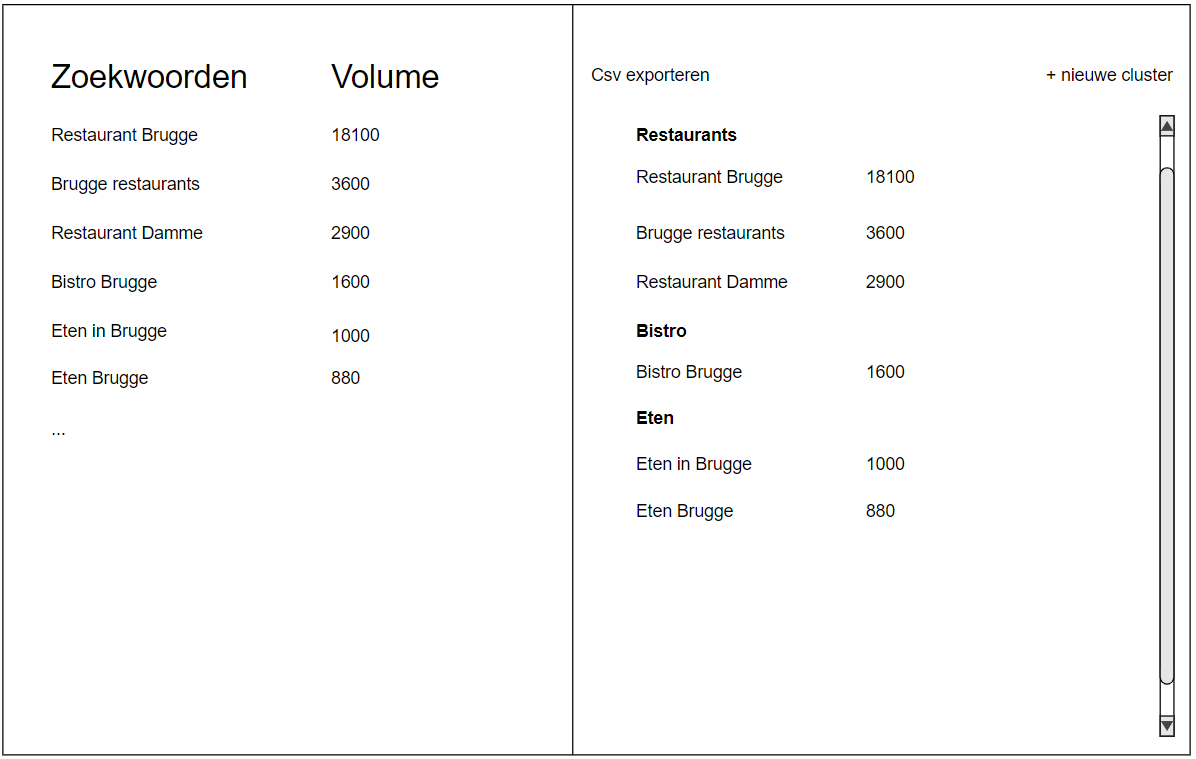
\includegraphics[width=0.8\textwidth]{img/Mockup2.png}
\caption{Screenshot van mock-up 2}
\end{figure}

Er staat een overzichtelijk scherm met alle zoekwoorden aan de linkerkant en een optie om clusters te creëren aan de rechterkant. Bij dit scherm krijgt de gebruiker de optie om een zoekwoord te selecteren en in de juiste cluster toe te voegen (of om eerst een nieuwe cluster aan te maken). 

Tot slot kan je als gebruiker al deze clusters met hun zoekwoorden exporteren naar een Csv- of Excel-bestand om verder te gebruiken. 

Op deze manier verricht je veel minder handmatig werk dan wanneer je alle zoekwoorden apart gaat kopiëren en plakken in een Spreadsheet of Excel-bestand. 

Er wordt dus vanaf nul een tool geprogrammeerd die voor een deel gebaseerd is op een bestaande tool. 

\section{Werking}
\label{ch: Werking}

\subsection{DataForSEO API}
\label{ch: DataForSEO API}

Om zoekwoordsuggesties en zoekvolumes te krijgen werd er gewerkt via een externe API. Via het online platform, DataForSEO, kon deze API geïntegreerd worden in het programma. 

Het programma is geschreven in de programmeertaal Java (Netbeans). Via deze documentatie, \textcite{DATAFORSEO}, wordt er aangetoond hoe de API in Java (Netbeans) geïmplementeerd kan worden. 

In de API-code kan je zelf verschillende elementen instellen: het zoekwoord waarvan je suggesties wil krijgen, het land, de taal en hoeveel zoekwoordsuggesties je wilt per zoekwoord. Deze code geeft dan gegevens zoals het zoekwoord, volume, ... terug in JSON-formaat. 

Bij de sectie 'related' worden de gerelateerde zoekwoorden (of zoekwoordsuggesties) gegeven. De meest relevante elementen die gebruikt worden zijn 'key' en 'search\_volume' omdat we bij de output enkel deze twee nodig hebben. 

Om de JSON-code te gebruiken in de applicatie, werd deze omgezet naar een Arraylist die door een MVC-applicatie (Model-View-Controller) gebruikt werd. 

\subsection{Model-View-Controller-Applicatie}
\label{ch: Model-View-Controller-Applicatie}

MVC-patroon staat voor Model-View-Controller-patroon. Dit patroon wordt gebruikt om de 'taken' te scheiden van de applicatie. 

'Model' staat voor een object met gegevens. Het kan ook een logica hebben om de controller bij te werken wanneer de gegevens veranderen. 

'View' vertegenwoordigt de visualisatie van de gegevens van het model. Het programma maakt gebruik van JavaFX Scenebuilder om het View-gedeelte op te bouwen. 

'Controller' werkt zowel op 'model' als op de 'View'. Het stuurt de datastroom naar het modelobject en werkt de weergave bij telkens wanneer de gegevens worden gewijzigd.

\subsubsection{Model-klasse}
\label{ch: Model-klasse}

Het JSON-bestand dat verkregen wordt via de API van DataForSEO wordt (in de Model-klasse) omgezet in een Arraylist (bijvoorbeeld met de volgende output: ["restaurant Brugge", 340; "Bistro Brugge", 250].)

Deze Arraylist wordt omgezet naar een Observablelist om te kunnen communiceren met de Controller (die aan de View gekoppeld is). 

\subsubsection{View-klassen}
\label{ch: View-klassen}

Er zijn in het programma twee View-klassen. Met behulp van het programma JavaFX Scenebuilder werden de twee schermen opgebouwd.

De eerste klasse is het startscherm waarbij de gebruiker drie waarden moet meegeven: de taal, het land en het zoekwoord waarvan er suggesties moeten gegeven worden. 

Het startscherm van de applicatie ziet er als volgt uit (opgemaakt in JavaFX Scenebuilder): 

\begin{figure}[h!]
\centering
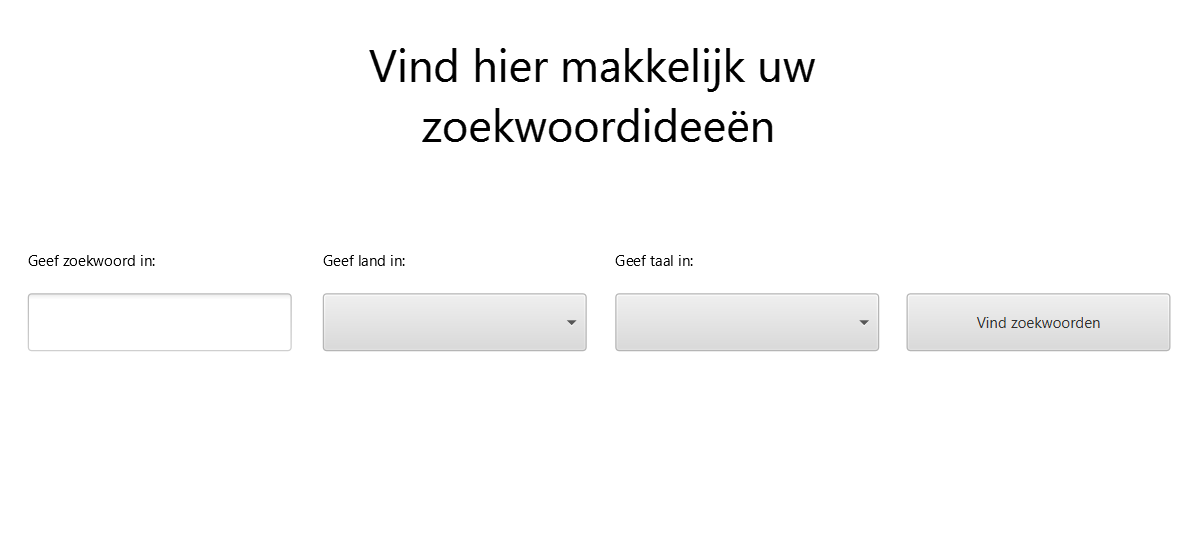
\includegraphics[width=0.8\textwidth]{img/keywordtoolscherm1.PNG}
\caption{Scherm 1 van de zelfgemaakte keywordtool}
\end{figure}

In het tekstvak (onder 'geef zoekwoord in:') kan je een zoekwoord ingeven zoals 'Restaurant Brugge' om zoekwoordsuggesties te krijgen. In de eerste dropdownlist kan je een land selecteren (België of Nederland) om het zoekwoordvolume te krijgen voor een specifiek land. In de rechtste dropdownlist (Onder 'Geef taal in:') kan je de taal kiezen van het zoekwoord, Nederlands of Engels. 

Deze drie waarden worden vervolgens (door op de knop 'vind zoekwoorden' te klikken) door middel van setters automatisch in de API-code geïntegreerd. Uit deze API-code wordt meteen de nodige JSON-code gegenereerd. 

De JSON-code wordt omgezet in leesbare taal voor de controller en er wordt een tableview gegenereerd met twee kolommen: de zoekwoorden met het maandelijks gemiddeld zoekvolume van de laatste 12 maanden (voor het gekozen land en taal). 

Nadat er op de knop 'Vind zoekwoorden' geklikt is heeft het scherm een linker- en rechterkant. Aan de linkerkant wordt een tableview (lijst) gegenereerd met de zoekwoordsuggesties en het bijhorende zoekvolume. 

\begin{figure}[h!]
\centering
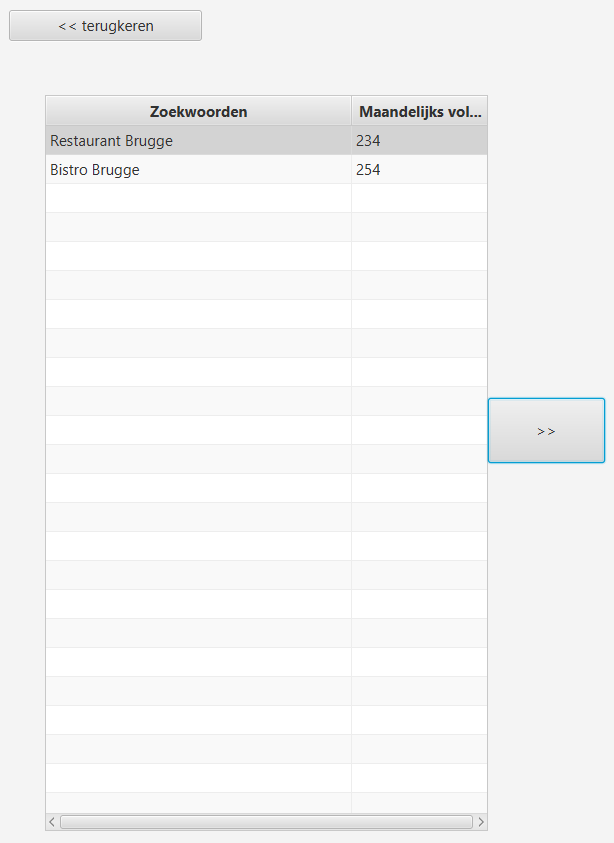
\includegraphics[width=0.8\textwidth]{img/scherm2linkerkant.PNG}
\caption{Scherm 2, linkerkolom van de zelfgemaakte tool}
\end{figure}

Bovenaan is er een knop om terug te keren naar de startpagina. De tableview van de linkerkolom wordt dan automatisch terug geledigd. 

Er staat een knop ( >> ) om de zoekwoorden van links naar rechts over te brengen. 

In de rechterkolom staat een tabel om de zoekwoorden en het zoekvolume van de linkerkolom in over te brengen. De tabel kan onderverdeeld worden in verschillende secties om de zoekwoorden en het zoekvolume te groeperen in clusters. 

Om een nieuwe sectie (of cluster) aan te maken, geef je de naam in van de sectie en druk je op de knop '+ cluster'. Binnen die sectie kan je dan zoekwoorden toevoegen.

Er staat een knop ( << ) om de zoekwoorden van de rechterkant terug over te brengen naar de linkerkant indien het zoekwoord toch niet nodig is in de lijst. 

Bovenaan staat een knop om de tableview te exporteren naar een Excel-bestand dat uiteindelijk kan geleverd worden aan de klant. 


\subsubsection{Controller-klassen}
\label{ch: Controller-klassen}

De Java-Applicatie heeft twee controller-klassen. Het startscherm heeft een controller-klasse die de ingevoerde waarden doorstuurt naar de API-klasse. Door middel van setters worden de waarden (zoekwoord, land en taal) correct ingesteld en wordt de JSON-code gegenereerd. 

Nadat de JSON-code is omgezet naar een Arraylist, worden de gegevens in een Tableview omgezet. De tweede controller-klasse is verantwoordelijk voor de Tableviews (linker- en rechterkant). 

\begin{figure}[h!]
\centering
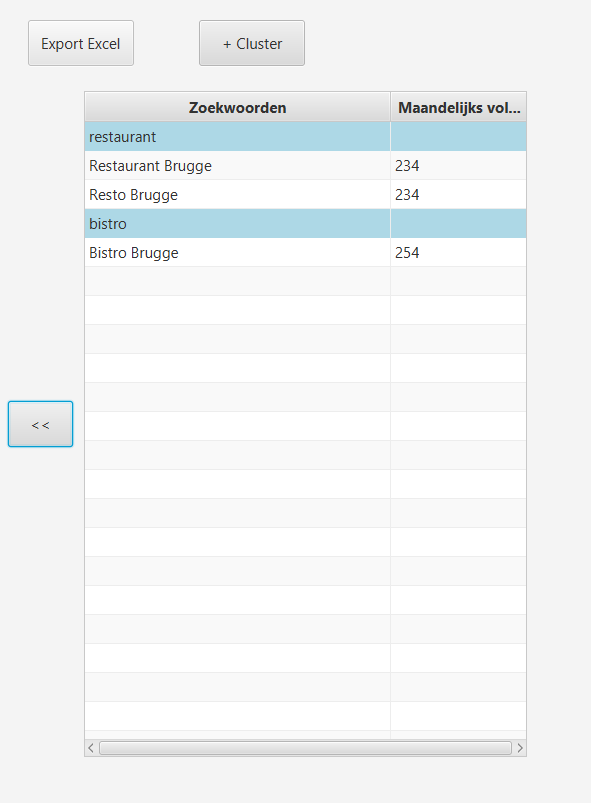
\includegraphics[width=0.8\textwidth]{img/scherm2rechterkant.PNG}
\caption{Scherm 2, rechterkolom van de zelfgemaakte tool}
\end{figure}